\documentclass[12pt]{article}
\usepackage[margin=2.5cm]{geometry}
\usepackage{enumerate}
\usepackage{amsfonts}
\usepackage{amsmath}
\usepackage{fancyhdr}
\usepackage{amsmath}
\usepackage{amssymb}
\usepackage{amsthm}
\usepackage{mdframed}
\usepackage{graphicx}
\usepackage{subcaption}
\usepackage{adjustbox}
\usepackage{listings}
\usepackage{xcolor}
\usepackage{booktabs}
\usepackage[utf]{kotex}

\definecolor{codegreen}{rgb}{0,0.6,0}
\definecolor{codegray}{rgb}{0.5,0.5,0.5}
\definecolor{codepurple}{rgb}{0.58,0,0.82}
\definecolor{backcolour}{rgb}{0.95,0.95,0.92}

\lstdefinestyle{mystyle}{
    backgroundcolor=\color{backcolour},
    commentstyle=\color{codegreen},
    keywordstyle=\color{magenta},
    numberstyle=\tiny\color{codegray},
    stringstyle=\color{codepurple},
    basicstyle=\ttfamily\footnotesize,
    breakatwhitespace=false,
    breaklines=true,
    captionpos=b,
    keepspaces=true,
    numbers=left,
    numbersep=5pt,
    showspaces=false,
    showstringspaces=false,
    showtabs=false,
    tabsize=1
}

\lstset{style=mystyle}

\begin{document}
\title{CSC236 Assignment 1}
\author{Hyungmo Gu}
\maketitle

\section*{Question 1}
\begin{enumerate}[a.]
    \item

    Yes. We can prove $P(235)$ follows from $P(234)$.

    \bigskip

    \begin{proof}
    Let $b$ be the bipartite graph with 235 vertices where
    117 vertices are in one partition and 118 vertices in
    the other partition (Note this is the configuration where maximum number of edges form).

    \bigskip

    The bipartite graph with 117 vertices on both sides of partition has
    $\frac{234^2}{4}$ edges, and the assumption tells us this is the maximum number of edges the
    bipartite graph could form.

    \bigskip

    Since we know $b$ has 117 more edges than the bipartite graph with 117 vertices on
    both sides, using these facts, we can conclude the upper bound number of edges for the bipartite
    graph with 235 vertices is

    \begin{align}
        \frac{234^2}{4} + 117 &= \frac{234^2}{4} + \frac{4 \cdot 117}{4}\\
        &= \frac{234^2 + 2 \cdot 234}{4}\\
        &\leq \frac{234^2 + 2 \cdot 234 + 1}{4}\\
        &= \frac{(234+1)^2}{4}\\
        &= \frac{(235)^2}{4}
    \end{align}

    \end{proof}

    \bigskip

    \begin{mdframed}
        \underline{\textbf{Attempt \#2:}}

        \bigskip

        Assume $P(234)$. That is, every bipartite graph on 234 vertices has no more
        than $\frac{234^2}{4}$ edges.

        \bigskip

        We need to prove $P(235)$ follows. That is, every bipartite graph on 235
        vertices has no more than $\frac{235^2}{4}$ edges.

        \bigskip

        Let $b$ be the bipartite graph with 235 vertices. Let $b'$ be the bipartite
        graph with a vertex removed from the larger of two partitions in $b$ along with its edges.

        \bigskip

        Since we know the maximum number of edges occur in $b'$ when there are
        117 vertices in both sides of the partitions, and since we know the edges
        of removed vertex forms edges with partition with bigger number of vertices,
        we can conclude the removed vertex forms at most 117 edges.

        \bigskip

        Since the assumption tells us $b'$ has at most $\frac{234^2}{4}$ edges,
        we can conclude the upper bound number of edges for the bipartite
        graph with 235 vertices is


        \begin{align}
            \frac{234^2}{4} + 117 &= \frac{234^2}{4} + \frac{4 \cdot 117}{4}\\
            &= \frac{234^2 + 2 \cdot 234}{4}\\
            &\leq \frac{234^2 + 2 \cdot 234 + 1}{4}\\
            &= \frac{(234+1)^2}{4}\\
            &= \frac{(235)^2}{4}
        \end{align}

        \bigskip

        So $P(235)$ follows.

    \end{mdframed}

    \bigskip

    \underline{\textbf{Notes:}}

    \bigskip

    \begin{itemize}
        \item I have a stuck feeling as to how I can formulate this kind of proof.
        \item 5+ hours spent on this problem
        \item I feel I wronged the proof by using existential quantifier
        \item Noticed professor generalized his statement instead of using bipartite
        with $x$ number of vertices in one partition and $y$ vertices in other partition
        example

        \begin{center}
        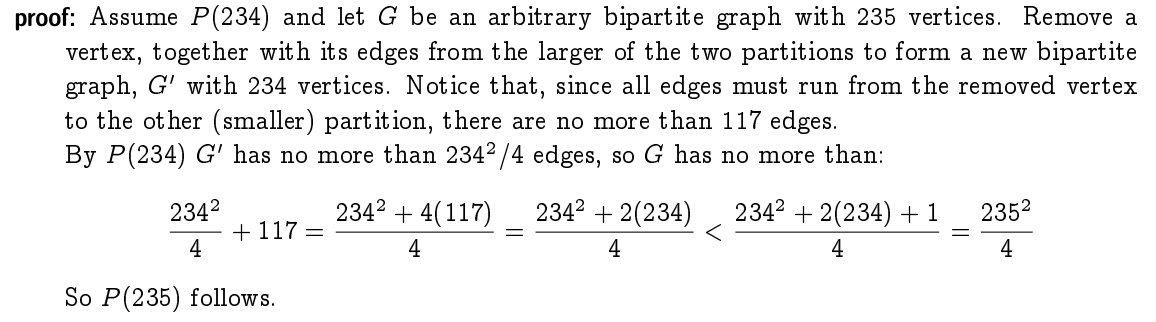
\includegraphics[width=0.8\linewidth]{images/assignment_1_q1a_note.png}
        \end{center}
    \end{itemize}

    % \bigskip

    % \begin{mdframed}
    %     \underline{\textbf{Rough Work:}}

    %     Assume $P(234)$. That is, every bipartite graph on 234 vertices has no more
    %     than $\frac{234^2}{4}$ edges.

    %     \bigskip

    %     We need to prove $P(235)$ follows. That is, every bipartite graph on 235
    %     vertices has no more than $\frac{235^2}{4}$ edges.

    %     \begin{enumerate}[1.]
    %         \item Find the configuration where bipartite graph on 235 vertices form most number of edges in
    %         terms of bipartite graph on 234 vertices.

    %         \begin{mdframed}
    %         Let $b$ be the bipartite graph with 235 vertices where
    %         117 vertices are in one partition and 118 vertices in
    %         the other partition (Note this is the configuration where maximum number of edges form).

    %         \end{mdframed}

    %         \item Show that $\frac{235^2}{4}$ is the most number of edges bipartite graph on 235
    %         vertices could form.

    %         \begin{mdframed}
    %         The bipartite graph with 117 vertices on both sides of partition has
    %         $\frac{234^2}{4}$ edges, and the assumption tells us this is the maximum number of edges the
    %         bipartite graph could form.

    %         \bigskip

    %         Since we know $b$ has 117 more edges than the bipartite graph with 117 vertices on
    %         both sides, using these facts, we can conclude the upper bound number of edges for the bipartite
    %         graph with 235 vertices is

    %         \begin{align}
    %             \frac{234^2}{4} + 117 &= \frac{234^2}{4} + \frac{4 \cdot 117}{4}\\
    %             &= \frac{234^2 + 2 \cdot 234}{4}\\
    %             &\leq \frac{234^2 + 2 \cdot 234 + 1}{4}\\
    %             &= \frac{(234+1)^2}{4}\\
    %             &= \frac{(235)^2}{4}
    %         \end{align}

    %         \bigskip
    %         \end{mdframed}
    %     \end{enumerate}

    % \end{mdframed}

    \item

    No. $P(236)$ doesn't follow from $P(235)$.

    \bigskip

    \begin{proof}
        Assume $P(235)$. That is, every bipartite graph with 235 vertices has no
        more than $\frac{235^2}{4}$ edges.

        \bigskip

        We need to show $P(236)$ doesn't follow. That is, there is a bipartite graph
        $b$ with 236 vertices that has more than $\frac{236^2}{4}$ edges.

        \bigskip

        Let $b$ be bipartite graph with 118 vertices in $V_1$ and 118 vertices in
        $V_2$ (Notice that this forms the most number of edges).

        \bigskip

        The assumption tells us that every bipartite graph with 235 vertices
        has $\frac{235^2}{4}$ edges.

        \bigskip

        Since we know that by removing a vertex with 118 edges from either one
        of the partition results in bipartite graph with 235 vertices, using
        above fact, we can write that $b$ has

        \setcounter{equation}{0}
        \begin{align}
            \frac{235^2}{4} + 118 = 13924.25
        \end{align}

        edges.

        \bigskip

        Since $\frac{236^2}{4} = 13924.0$, we can conclude $P(236)$ doesn't follow.

    \end{proof}

    \bigskip

    \underline{\textbf{Notes:}}

    \begin{itemize}
        \item Noticed that professor tried to show the bipartite graph with
        234 vertices with 117 vertices in $V_1$ and 117 vertices in $V_2$ is the
        one and the only bipartite graph with 234 vertices that form the most number of edges.
    \end{itemize}

    % \bigskip

    % \begin{mdframed}
    %     \underline{\textbf{Rough Work:}}

    %     \bigskip

    %     Assume $P(235)$. That is, every bipartite graph with 235 vertices has no
    %     more than $\frac{235^2}{4}$ edges.

    %     \bigskip

    %     We need to show $P(236)$ doesn't follow. That is, there is a bipartite graph
    %     $b$ with 236 vertices that has more than $\frac{236^2}{4}$ edges.

    %     \bigskip

    %     Let $b$ be bipartite graph with 118 vertices in $V_1$ and 118 vertices in
    %     $V_2$ (Notice that this forms the most number of edges).

    %     \begin{enumerate}[1.]

    %         \item Show that this is 118 edges more than $\frac{235^2}{4}$.

    %         \begin{mdframed}

    %         The assumption tells us that every bipartite graph with 235 vertices
    %         has $\frac{235^2}{4}$ edges.

    %         \bigskip

    %         Since we know that by removing a vertex with 118 edges from either one
    %         of the partition results in bipartite graph with 235 vertices, using
    %         above fact, we can write that $b$ has

    %         \begin{align}
    %             \frac{235^2}{4} + 118 = 13924.25
    %         \end{align}

    %         edges.

    %         \end{mdframed}

    %         \item Conclude this choice of $b$ has more than $\frac{236^2}{4}$ edges.
    %         \begin{mdframed}
    %         Since $\frac{236^2}{4} = 13924.0$, we can conclude $P(236)$ doesn't follow.
    %         \end{mdframed}
    %     \end{enumerate}

    %     \bigskip

    %     \begin{mdframed}
    %         Assume $P(235)$. That is, every bipartite graph with 235 vertices has no
    %         more than $\frac{235^2}{4}$ edges.

    %         \bigskip

    %         We need to show $P(236)$ doesn't follow. That is, there is a bipartite graph
    %         $b$ with 236 vertices that has more than $\frac{236^2}{4}$ edges.

    %         \bigskip

    %         Let $b$ be bipartite graph with 118 vertices in $V_1$ and 118 vertices in
    %         $V_2$ (Notice that this forms the most number of edges).

    %         \bigskip

    %         The assumption tells us that every bipartite graph with 235 vertices
    %         has $\frac{235^2}{4}$ edges.

    %         \bigskip

    %         Since we know that by removing a vertex with 118 edges from either one
    %         of the partition results in bipartite graph with 235 vertices, using
    %         above fact, we can write that $b$ has

    %         \begin{align}
    %             \frac{235^2}{4} + 118 = 13924.25
    %         \end{align}

    %         edges.

    %         \bigskip

    %         Since $\frac{236^2}{4} = 13924.0$, we can conclude $P(236)$ doesn't follow.
    %     \end{mdframed}

    % \end{mdframed}

    \item

    \bigskip

    \begin{mdframed}
        \underline{\textbf{Rough Work:}}

        \bigskip

        For convenience, define

        \begin{align*}
        & H(n):\:\text{Every bipartite graph with $n$ vertices has no more than
        $\frac{(n-1)^2}{4}$ edges}\\
        & \text{when $n$ is odd, or $\frac{n^2}{4}$ edges when $n$ is even.}
        \end{align*}

        \bigskip

        I must prove $\forall n \in \mathbb{N}$, $H(n)$.

        \bigskip

        \begin{enumerate}[1.]
            \item Base Case ($n = 0$)

            \bigskip

            We need to show $H(0)$. That is, every bipartite graph with 0 vertices
            has no more than 0 edges.

            \bigskip

            \begin{itemize}
                \item State that bipartite graph with 0 vertices has 0 edge.
                \item Conclude that $H(n)$ is verified.
            \end{itemize}

            \item Inductive Step
        \end{enumerate}

    \end{mdframed}
\end{enumerate}

\bigskip

\underline

\section*{Question 2}

\section*{Question 3}

\section*{Question 4}

\end{document}